\chapter{高阶笼上的柯西–格林坐标：闭式解析}
% 旧版合并草稿：当前不再由 main.tex 引用。
% 现行第3章与第5章分别见 chapters/Chap3_query.tex 与 chapters/Chap5_cauchy.tex。

% ===== Chapter 4 macros =====
\providecommand{\Bezier}{B\'{e}zier }
\providecommand{\tr}[1]{#1}
\providecommand{\tb}[1]{#1}
\providecommand{\todo}[1]{}
\providecommand{\argmin}{\mathop{\mathrm{arg\,min}}\limits}
\providecommand{\argmax}{\mathop{\mathrm{arg\,max}}\limits}
\providecommand{\res}{\mathop{\mathrm{Res}}}
\providecommand{\re}{\mathop{\mathrm{Re}}}
\providecommand{\im}{\mathop{\mathrm{Im}}}

\makeatletter
\@ifundefined{theorem}{\newtheorem{theorem}{Theorem}}{}
\@ifundefined{lemma}{\newtheorem{lemma}{Lemma}}{}
\@ifundefined{prop}{%
  \@ifundefined{theorem}{%
    \newtheorem{prop}{Proposition}[chapter]%
  }{%
    \newtheorem{prop}[theorem]{Proposition}%
  }%
}{}
\makeatother

\def \ma {\mathbf{a}}
\def \me {\mathbf{e}}
\def \mb {\mathbf{b}}
\def \mc {\mathbf{c}}
\def \md {\mathbf{d}}
\def \mf {\mathbf{f}}
\def \mg {\mathbf{g}}
\def \mh {\mathbf{h}}
\def \mi {\mathbf{i}}
\def \mj {\mathbf{j}}
\def \mk {\mathbf{k}}
\def \ml {\mathbf{l}}
\def \mm {\mathbf{m}}
\def \mn {\mathbf{n}}
\def \mo {\mathbf{o}}
\def \mp {\mathbf{p}}
\def \mq {\mathbf{q}}
\def \mr {\mathbf{r}}
\def \ms {\mathbf{s}}
\def \mt {\mathbf{t}}
\def \muu {\mathbf{u}}
\def \mv {\mathbf{v}}
\def \mw {\mathbf{w}}
\def \mx {\mathbf{x}}
\def \my {\mathbf{y}}
\def \mz {\mathbf{z}}

\section{概述}\label{sec:chap4-overview}
笼坐标为在二维区域上定义标量场或向量场提供了统一方式：用户只需在边界上给定稀疏约束，即可将其传播到整个内部区域。
由于具有直观的边界控制能力，这类方法已被广泛用于二维形状变形、图像着色和艺术编辑等任务。
现有笼坐标大致可分为两类：一类通过边界顶点值的加权组合实现插值，如均值坐标、正均值坐标与调和坐标~\cite{Floater2003,Hormann2006,Lipman2007,Joshi2007}；另一类进一步引入边界导数信息，如 Green 坐标与 Cauchy 坐标~\cite{Lipman2008,Weber2009}。
其中，Green 坐标与 Cauchy 坐标在二维情形下都与保角形变密切相关，因此在形状保持方面具有明显优势。

近年来，三次均值坐标、多项式 Green 坐标和多项式 Cauchy 坐标等工作开始支持将初始直边笼变形为高阶多项式曲线~\cite{Li2013,MichelThiery2023,Lin2024PolynomialCC}。
但这些方法在编码阶段仍建立在线性输入笼之上。
当输入形状本身具有明显的曲边特征时，线性笼通常需要大量边段才能贴合轮廓，这不仅降低了交互操控的直观性，也容易影响边界附近的形变光滑性。
为此，我们关注由多项式曲线组成的输入笼，并将其称为高阶笼。
与线性笼相比，高阶笼能够更紧密地逼近原始形状，以更少的参数表达边界；同时，多项式边界与 CAD 中常见的自由形状设计方式更一致，更适合作为直接的编辑界面；此外，高阶笼得到的变形在边界附近也更光滑。

尽管已有工作将 Cauchy 坐标推广到高阶笼~\cite{Lin2024PolynomialCC}，但其仍需借助中间线性笼，并通过数值方式计算从中间笼到输入笼映射的逆映射。
这带来两个问题：其一，坐标及其导数缺乏闭式表达，难以直接支持点到点变形；其二，高阶输入笼需要满足较强且不够直观的几何约束，因此难以处理任意有效的高阶包围边界。
围绕这一问题，本章前半部分给出二维高阶笼上的 Cauchy 坐标及其导数的闭式形式。
核心在于将相关积分转化为有理多项式积分，并结合对数函数与留数定理构造可计算的解析表达；同一积分框架还可扩展到高阶笼上的 Green 坐标。

在此基础上，本章后半部分进一步讨论另一类与曲边边界密切相关的闭式计算问题，即 \Bezier 曲线广义环绕数及其导数的解析求值。
接下来，第~\ref{sec:cau-method} 节给出高阶笼上的 Cauchy 坐标推导、闭式解、扩展与实现细节，第~\ref{sec:cau-results} 节展示其在基于笼变形和点到点变形中的效果与对比实验。
随后，第~\ref{sec:qry-method} 节讨论 \Bezier 曲线广义环绕数、边界点情形及导数计算，第~\ref{sec:qry-results} 节展示其在曲线查询中的数值评估。

\section{方法（柯西坐标）} \label{sec:cau-method}
我们先在第~\ref{sec:cau-revisit} 节回顾 Cauchy 坐标，再在第~\ref{sec:cau-High-order-Cauchy} 节介绍高阶笼上的 Cauchy 坐标，最后在第~\ref{sec:cau-closed-form} 节推导这些坐标及其导数的闭式表达。
%
更多讨论见第~\ref{sec:cau-connection} 与第~\ref{sec:cau-details} 节。

\subsection{回顾 Cauchy 坐标}\label{sec:cau-revisit}
\paragraph{Cauchy 变换}
作为复分析中的基础结论，Cauchy 积分公式指出：定义在平面区域 \(\Omega\) 上、且边界 $\partial \Omega$ 为简单闭曲线的全纯函数，可由其在 $\partial \Omega$ 上的取值完全决定。
%
将连续函数 \(f\) 的边界值代入 Cauchy 积分公式右侧，可得到一个全纯函数 \(u\)：
\begin{equation}\label{equ:cau-Cauchy-integral}
    u(z)=\frac{1}{2\pi i}\int_{\partial \Omega}\frac{f(\zeta)}{\zeta-z} d\zeta,\ \ z \in \Omega,
\end{equation}
其中 $z$ 为复数，且 \(i=\sqrt{-1}\)。
这种从 \(f\) 到 \(u\) 的变换称为\emph{Cauchy 变换} \cite{Bell2015cauchytransform}。
文献中的两类 Cauchy 坐标~\cite{Weber2009,Lin2024PolynomialCC} 均来源于该变换。

\paragraph{笼（Cage）}
给定有界区域 $\Omega$，其边界 $\partial \Omega$（即\emph{笼}）是一个无自交闭合曲线，由顶点集 $V = \{\mv_j\}^n_{j=1}$ 和边集 $E = \{\me_j\}^n_{j=1}$ 组成（按逆时针定向），见图~\ref{fig:cau-notations}。
%
在复平面上，每个顶点 $\mv_j$ 记作复数 \(z_j=\mv_{j,x}+\mv_{j,y} i\)。
%
Cauchy 坐标~\cite{Weber2009} 与多项式 Cauchy 坐标~\cite{Lin2024PolynomialCC} 都定义在具有直边的初始笼上，即对边 $\me_j = \overline{\mv_{j-1}\mv_j}$，有 \( z_{\me_j}(t) = (1-t) z_{j-1} + t z_j,\ t\in[0,1]\)。
二者的区别在于变形后笼边的表示：
\begin{itemize}
    \item 对 Cauchy 坐标，新的 $\me_j$ 为线段，即 $f^\text{new}(z_{\me_j}(t)) = (1-t) p^\text{new}_{j-1}+t p^\text{new}_{j}$，其中 $p^\text{new}_{j}$ 为顶点 $\mv_j$ 的新位置。
    \item 对多项式 Cauchy 坐标，新的 $\me_j$ 为次数 $n_j \geq 1$ 的多项式曲线，即 $f^\text{new}(z_{\me_j}(t)) = \sum_{k=0}^{n_j} B^{n_j}_k(t) p^\text{new}_{\me_j,k}$，其中 $B^{n_j}_k (t)$ 为 Bernstein 多项式，$p^\text{new}_{\me_j,k} \in \mathbb{C}$ 为控制点。
\end{itemize}
由于多项式情形包含线性情形（$n_j = 1$），下文仅讨论多项式 Cauchy 坐标。

\paragraph{Cauchy 坐标推导}
将变形笼的新位置代入式~\eqref{equ:cau-Cauchy-integral}，可得
\begin{equation}\label{equ:cau-discretization}
\begin{split}
    u(z) &:=\frac{1}{2\pi i} \sum_{j=1}^n \int_{\me_j}\frac{f^\text{new}(\zeta)}{\zeta-z}d\zeta \\
     &=\frac{1}{2 \pi i}\sum_{j=1}^n \sum_{k=0}^{n_j} \left(\int_{\me_j}\frac{B^{n_j}_k (t)}{\zeta-z}d\zeta\right) p^\text{new}_{\me_j,k}, \ \ z \in \Omega.
\end{split}
\end{equation}
用户通过编辑控制点 $p^\text{new}_{\me_j,k}$ 可直观地完成形变。
此外，在式~\eqref{equ:cau-discretization} 中，与控制点 $p^\text{new}_{\me_j,k}$ 对应的全部积分项（$\frac{1}{2 \pi i}\left(\int_{\me_j}\frac{B^{n_j}_k (t)}{\zeta-z}d\zeta\right)$）共同构成其 Cauchy 坐标~\cite{Lin2024PolynomialCC}。
由于 $B^{n_j}_k (t) = 
\begin{pmatrix}
n_j \\
k \\
\end{pmatrix}
t^k (1-t)^{n_j-k}$，
我们只需评估不同 $k$ 下的积分 $\left(\int_{\me_j}\frac{t^k}{\zeta-z}d\zeta\right)$ 即可得到坐标。

\begin{figure}[t]
  \centering
   \vspace{-2mm}
  \begin{overpic}[width=0.99\linewidth]{figures/chap4_notation.pdf}
    {
 \put(31,9){\small $\me_j$}
 \put(40,19){\small $\zeta$}
 \put(13,13.5){\small $\Omega$}
 \put(23,23.5){\small $z$}
 \put(50,24){\small $u$}
 \put(80,23.5){\small $u(z)$}
 \put(91,7){\small $f^{\text{new}}(\me_j)$}
    }
  \end{overpic}
  \vspace{-5mm}
  \caption{
  高阶笼变形示意。原始曲线 $\me_j$ 变形为 $f^{\text{new}(\me_j)}$，笼内任意点 $z$ 变形为 $u(z)$。
  }
  \label{fig:cau-notations}
\end{figure}

\subsection{高阶笼上的二维 Cauchy 坐标及其导数}\label{sec:cau-High-order-Cauchy}

\paragraph{更强的变形交互性}
由 Cauchy 积分公式可得
\begin{equation}
    u(z)-z=\frac{1}{2\pi i}\int_{\partial \Omega}\frac{f(\zeta)-\zeta}{\zeta-z} d\zeta,\ \ z \in \Omega,
\end{equation}
其中 \(f(\zeta)-\zeta\) 表示笼边界点 $\zeta$ 的位移（通常非全纯），而 \(u(z)-z\) 为内部点 \(z\) 的形变位移。
由于 \(u(z)-z\) 是全纯函数，依据最大模原理，其最大位移出现在 \(\partial \Omega\) 上。
因此，对同一边界位移场而言，离笼越近的区域形变位移越大，边界附近交互性更强。
这也是为何在交互编辑中，通常希望笼尽可能贴近形状，而非采用远离形状的大包围边界。
高阶笼相比线性笼具有更强逼近能力，因此我们将 Cauchy 坐标推广到高阶输入笼。

\paragraph{边界上的全纯性}
Cauchy 坐标与多项式 Cauchy 坐标都能在 \(\Omega\) 内生成全纯函数 $u$。
若全纯函数导数不为 0，则其为保角映射，因此可得到保角形变。
但 $u$ 在 \(\partial \Omega\) 上一般并非全纯，这会导致边界附近不够光滑（见 \cite{Lin2024PolynomialCC} 图 4）。
若输入二维形状仅由直边构成，则可由初始线性笼紧密逼近；这时，多项式 Cauchy 坐标可通过将直边变形为 \Bezier 曲线来获得更平滑结果，其依据是以下定理：
\begin{theorem}[Theorem 3.3 in \cite{Bell2015cauchytransform}]\label{pro:cau-holomorphic}
设 \(\partial \Omega\) 光滑，且 \(u\) 是定义在 \(\Omega\) 上的全纯函数，并可延拓为 \(\Omega\cup \partial \Omega\) 上的连续函数。若 \(u\) 的边界值在 \(\partial\Omega\) 的某条开弧 \(\Gamma\) 上光滑，则 \(u\) 的各阶导数都可由 \(\Omega\) 连续延拓到 \(\Omega \cup \Gamma\)。
\end{theorem}

然而，对于曲边形状若仍使用线性输入笼，边界非全纯问题依旧存在（图~\ref{fig:cau-cmp-smoothness}）。
幸运的是，定理~\ref{pro:cau-holomorphic} 也表明：若变形前后某条边都光滑，则 $u$ 在该边界处可保证全纯。
这推动我们将 Cauchy 坐标推广到高阶输入笼，使其能用光滑边更紧密包围输入形状。
假设 \(\partial \Omega\) 为分段光滑边界，可由定理~\ref{pro:cau-holomorphic} 直接推出：
 \begin{lemma}\label{pro:cau-lemma_holo}
 全纯函数 \(u\) 在 \(\partial \Omega\) 上全纯，当且仅当 \(f\) 将边界的光滑段映射到光滑段，且 \(f\) 在非光滑顶点处为相似变换。
 \end{lemma}

\paragraph{推导}
现在我们将 Cauchy 坐标扩展到由多项式曲线组成的高阶初始笼 $\partial \Omega$。
输入边 $\me_j$ 表示为次数 $m_j \geq 1$ 的 \Bezier 曲线：$z_{\me_j}(t) = \sum^{m_j}_{k=0} B_k^{m_j}(t) p^\text{old}_{\me_j,k} , \forall t \in [0, 1]$，其中 $p^\text{old}_{\me_j,k} \in \mathbb{C}$ 为控制点。
不失一般性，仍假设 $\me_j$ 的变形曲线为 $f^\text{new}(z_{\me_j}(t)) = \sum_{k=0}^{n_j} B^{n_j}_k(t) p^\text{new}_{\me_j,k}$。
则有
\begin{equation}\label{equ:cau-discrete-curved}
\begin{split}
    u(z) &=\frac{1}{2\pi i} \sum_{j=1}^n \int_{\me_j}\frac{f^\text{new}(\zeta)}{\zeta-z}d\zeta \\
    &= \frac{1}{2\pi i} \sum_{j=1}^n \int^1_{0} \frac{\sum_{k=0}^{n_j} p^\text{new}_{\me_j,k} B^{n_j}_k(t) z'_{\me_j}(t)}{z_{\me_j}(t) - z} dt \\
     &= \frac{1}{2\pi i} \sum_{j=1}^n \sum_{k=0}^{n_j} \left(\int^1_{0} \frac{ B^{n_j}_k(t) z'_{\me_j}(t)}{z_{\me_j}(t) - z} dt \right) p^\text{new}_{\me_j,k}, \ \ z \in \Omega.
\end{split}
\end{equation}
我们将式~\eqref{equ:cau-discrete-curved} 括号内积分记为 $\alpha_{\me_j,k}(z)$。
与控制点 $p^\text{new}_{\me_j,k}$ 相关的所有积分共同组成其 Cauchy 坐标。

\begin{equation}\label{equ:cau-derivative-curved}
     \frac{d^l \alpha_{\me_j,k}(z)}{ dz^l } = l! \int^1_{0} \frac{ B^{n_j}_k(t) z'_{\me_j}(t)}{(z_{\me_j}(t) - z)^{l+1}} dt.
\end{equation}
该式使坐标导数可直接计算。

\begin{figure}[t]
  \centering
  \begin{overpic}[width=0.99\linewidth]{figures/chap4_smooth_poly.pdf}
    {
 \put(16,-2){\small \textbf{(a1)}}
 \put(40,-2){\small \textbf{(a2)}}
 \put(67,-2){\small \textbf{(b1)}}
 \put(89,-2){\small \textbf{(b2)}}
    }
  \end{overpic}
  \vspace{-1mm}
  \caption{
  多项式 Cauchy 坐标将线性笼（a1，边上非端点控制点以实点表示）映射到三次笼时，边界附近会出现不光滑（a2）。
  我们的三次输入笼可紧密包围形状（b1），并得到光滑形变（b2）。
  }
  \label{fig:cau-cmp-smoothness}
\end{figure}

\subsection{闭式解}\label{sec:cau-closed-form}
式~\eqref{equ:cau-discrete-curved}（坐标）和式~\eqref{equ:cau-derivative-curved}（坐标导数）中的被积函数均为有理多项式。
我们接下来给出该类积分的解析解计算方法，这是本文核心贡献。

\paragraph{表示方式}
将分母记为 $h(t), t\in[0,1]$，其次数为 $l$。
分子写为次数 $r$ 的多项式：$g(t) = \sum^r_{k=0} a_k t^k$，其中 $a_k$ 为系数。
由于 $\int^1_{0} g(t) / h(t) dt = \sum^r_{k=0} a_k \int^1_{0} t^k / h(t) dt$，我们只需计算 $\int^1_{0} t^k / h(t) dt, \forall k \geq 0$。

\paragraph{定理}
\begin{theorem}\label{pro:cau-general}
多项式 $h(t)$ 有 $m\leq l$ 个互异根 $\{\zeta_j\}^m_{j=1}$（$\zeta_j$ 为复数）。
则
$$\int_0^1 \frac{t^k}{ h(t)}dt=\sum_{j=1}^{m}\res(S_k(\zeta),\zeta_j), \zeta \in \mathbb{C}, $$
其中 $S_k(\zeta)=s_k(\zeta)/h(\zeta)$，且
$$s_k(\zeta)=\zeta^k(\log(1-\frac{1}{\zeta})+\sum_{j=1}^k\frac{1}{j \zeta^j}).$$
\end{theorem}

\begin{figure}[!t]
  \centering
  \begin{overpic}[width=0.5\linewidth]{figures/chap4_cauchy_complex.pdf}
    {
 \put(63,19){\small $\zeta_i$}
 \put(52,70){\small $\zeta_j$}
 \put(65,54){\small $l_1$}
 \put(50,40){\small $l_2$}
 \put(27,36){\small $0$}
 \put(85,36){\small $1$}
 \put(85,58){\small $\gamma_2$}
 \put(27,58){\small $\gamma_1$}
 \put(84,80){\small $\Gamma$}
    }
  \end{overpic}
  \vspace{-3mm}
  \caption{复平面上的积分路径。}
  \label{fig:cau-inte_path}
\end{figure}

\begin{proof}
我们考虑函数 \(S_k(\zeta)\) 沿积分路径（见图~\ref{fig:cau-inte_path}）的积分。
该路径由 \(\gamma_1,l_1,\gamma_2,l_2,\Gamma\) 组成，其中 \(\gamma_1,\gamma_2\) 分别是以 0 与 1 为圆心、半径为 \(\epsilon\) 的小圆，\(l_1,l_2\) 分别是线段 \([0,1]\) 的上、下侧，\(\Gamma\) 是半径为 \(R\) 的大圆（本证明令 \(R \to \infty\)）。

\(S_k(\zeta)\) 在该积分路径上全纯。
事实上，\(\log\left(1 - \frac{1}{\zeta}\right) = \log(1-\zeta) - \log(-\zeta)\)。
当 \(\zeta\) 沿任意绕过线段 \([0,1]\) 的简单闭曲线转一圈时，$\log\left(1 - \frac{1}{\zeta}\right)$ 仍保持单值全纯分支。
%
对 $S_k$ 在路径包围区域应用\emph{留数定理}，有
    \begin{equation}\label{equ:cau-residue_theorem}
        \begin{aligned}
 \int_{\gamma_1+l_1+\gamma_2+l_2+\Gamma} S_k(\zeta) \, d\zeta
            = 2\pi i \sum_{j=1}^{m} \res(S_k(\zeta), \zeta_j).
        \end{aligned}
    \end{equation}
当 $\zeta\in l_1$ 时，$\log(1-\zeta)-\log(-\zeta)=\log(1-t)+2 \pi i-\log(-t)$；
当 $\zeta\in l_2$ 时，$\log(1-\zeta)-\log(-\zeta)=\log(1-t)-\log(-t)$，其中 $t$ 为 $\zeta$ 的实部。
于是
\begin{equation}\label{equ:cau-l1l2}
\begin{aligned}
    &\int\limits_{l_1+l_2} S_k(\zeta) \, d\zeta=\int_{0}^1 \left(S_k(t) +\frac{2\pi i t^k}{h(t)}\right)\, dt+\int_1^0 S_k(t) \, dt\\
    &=2\pi i \int_{0}^{1} \frac{ t^k}{h(t)} \, dt.
    \end{aligned}
\end{equation}
 当 \( \zeta \in \Gamma \) 时，根据泰勒展开，\( s_k \) 可写为
    \begin{equation}
        s_k(\zeta)=\zeta^k(\sum_{j=1}^{\infty}\frac{-1}{j \zeta^j}+\sum_{j=1}^k\frac{1}{j \zeta^j})=\sum_{j=1}^\infty\frac{-1}{(k+j) \zeta^{j}}.
    \end{equation}
    由于 $h(\zeta)$ 次数至少为 1，有 $\lim_{R\to \infty}\zeta S_k(\zeta)=0$，从而
    \begin{equation}\label{equ:cau-Gamma}
        \lim\limits_{R\to \infty}\int_{\Gamma} S_k(\zeta) \, d\zeta=0.
    \end{equation}
    当 $\zeta \in \gamma_1$ 时，有
    \begin{equation}
    \begin{aligned}
       \lim\limits_{\epsilon\to 0} &\int_{\gamma_1} S_k(\zeta) \, d\zeta=\lim\limits_{\epsilon\to 0}\int_{\gamma_1} \frac{\zeta^k \log(-\zeta)}{h(\zeta)}\, d\zeta.\\
       &\leq \frac{\epsilon^k (-\log(\epsilon)+2 \pi)}{h(0)}2 \pi \epsilon \to 0.
       \end{aligned}
    \end{equation}
    对 $\zeta \in \gamma_2$ 同理，因此
    \begin{equation}\label{equ:cau-gamma12}
       \lim\limits_{\epsilon\to 0} \int_{\gamma_1+\gamma_2} S_k(\zeta) \, d\zeta=0.
    \end{equation}

    将~\eqref{equ:cau-l1l2}、\eqref{equ:cau-Gamma}、\eqref{equ:cau-gamma12} 代入~\eqref{equ:cau-residue_theorem}，即可得到
    \begin{equation}
        \int_0^1 \frac{t^k}{ h(t)}dx=\sum_{j=1}^{m}\res(S_k(\zeta),\zeta_j).
    \end{equation}
\end{proof}

\paragraph{说明}
在上述证明中，$\log(1-\zeta) - \log(0-\zeta)$ 将积分区间限定为 \([0,1]\)，额外项 $\sum \frac{1}{j \zeta^j}$ 用于保证 \(S_k\) 在无穷远点的留数为 0。
该定理也可扩展到区间 \([a,b]\) 的积分，只需把 $s_k(\zeta)$ 中对数项改写为 \(\log(b-\zeta)-\log(a-\zeta)\)，并保持附加项为该对数项泰勒展开前 $k$ 项的相反数。

\paragraph{一般根}
在最一般情形下，\( \zeta_j \) 是 \( S_k(\zeta) \) 的单极点。记 $h^{j,1}(\zeta)=h(\zeta)/(\zeta-\zeta_j)$，则
\begin{equation}\label{equ:cau-gene_expression}
\begin{aligned}
    &\res(S_k(\zeta),\zeta_j)=\lim_{\zeta\to \zeta_j}(\zeta-\zeta_j)S_k(\zeta)=\frac{s_k(\zeta_j)}{h^{j,1}(\zeta_j)}.
    \end{aligned}
\end{equation}

\paragraph{重根}
在计算 \(\alpha_{\me_j,k}(z)\) 时，少量点会出现多重极点。
例如，当输入边 $\me_j$ 为二次曲线时，多重极点意味着 \(z\) 与 $\me_j$ 的焦点重合。
此时记 \( \zeta_j \) 为 $l_j$ 阶极点，且 $h^{j,l_j}(\zeta)=h(\zeta)/(\zeta-\zeta_j)^{l_j}$，有
\begin{equation}\label{equ:cau-repeated_expression}
\begin{aligned}
&\res(S_k(\zeta),\zeta_j)
    =\lim_{\zeta\to \zeta_j}\frac{1}{(l_j-1)!}\frac{d^{l_j-1}}{d\zeta^{l_j-1}}\{\frac{s_k(\zeta)}{h^{j,l_j}(\zeta)}\}.
    \end{aligned}
\end{equation}
对给定 $l_j$，按标准求导规则即可计算。
在我们的实际计算中，尚未遇到计算 \(\alpha_{\me_j,k}(z)\) 时 $l_j>1$ 的情形。

\subsection{扩展}\label{sec:cau-connection}
\paragraph{多项式 Green 坐标}
\citet{MichelThiery2023} 提出了闭式多项式 Green 坐标，可将直边输入笼变形为曲边输出笼；但其不能处理高阶输入笼。
我们在其基础上利用本文定理，将 Green 坐标扩展到高阶笼。
根据~\cite{MichelThiery2023} 的式 (12)，高阶笼 Green 坐标计算可归结为如下积分：
定理~\ref{pro:cau-general} 可直接用于该积分。

\paragraph{有理多项式笼}
我们还可将坐标扩展到由有理多项式曲线构成的初始高阶笼 $\partial \Omega$（图~\ref{fig:cau-rational}）。
令 $z_{\me_j}(t) = \frac{z_{w,\me_j}(t)}{w(t)}, \forall t \in [0, 1]$，其中 \(z_{w,\me_j}(t)=\sum_{k=0}^{m_j}w_{\me_j,k}p_{\me_j,k}^{\text{old}}B_k^{n_j}(t)\)，\(w(t)=\sum_{k=0}^{m_j}w_{\me_j,k}B_k^{n_j}(t)\)。
随后将 $f^\text{new}(z_{\me_j}(t))$ 写为与其共享权重、控制点为新控制点 \(p^\text{new}_{\me_j,k}\) 的有理曲线，可得
\begin{equation}
    \alpha_{\me_j,k}(z)=\int_0^1 \frac{z_{w,\me_j}'(t)w(t)-w'(t)z_{w,\me_j}(t)}{(z_{w,\me_j}(t)-zw(t))w(t)^2}dt.
\end{equation}
定理~\ref{pro:cau-general} 同样可用于该积分。
当 \(w(t)\) 与 \(z_{\me_j}^{w}(t)-zw(t)\) 的根重合时，需要额外处理：实践中我们以误差阈值 \(\epsilon=10^{-10}\) 合并根后重新评估其重数。

\subsection{实现细节}\label{sec:cau-details}
算法~\ref{alg:cau-encoding} 给出了我们 Cauchy 坐标计算伪代码。

\paragraph{计算 \(\{\zeta_j\}\)}
为应用定理~\ref{pro:cau-general} 计算高阶笼 Cauchy 坐标，需要先求解 $h(t)=0$ 的根 $\{\zeta_j\}$。
对最常用的二次和三次曲线，可使用闭式求根公式。
对四次以上多项式，则需数值求根。

\paragraph{递推计算}\label{sec:cau-encoding}
我们以迭代方式计算 \(\res(S_{k}(\zeta),\zeta_j)\)。为简洁起见，仅给出 \(\zeta_j\) 为单极点的情形（多极点类似）。
由
    $s_{k+1}(\zeta)=\zeta s_k(\zeta)+\frac{1}{k+1},\ k\geq 0,$
在实践中使用如下递推：
\begin{equation}\label{equ:cau-recur}
\begin{aligned}
&\res(S_{0}(\zeta),\zeta_j)=\frac{s_0(\zeta_j)}{h^{j,1}(\zeta_j)},\\
    &\res(S_{k+1}(\zeta),\zeta_j)=\zeta_j \res(S_k(\zeta),\zeta_j)+\frac{1}{k+1}\frac{1}{h^{j,1}(\zeta_j)}.
    \end{aligned}
\end{equation}

\begin{algorithm}[t]
  \caption{计算初始位置点 $z$ 的 Cauchy 坐标}\label{alg:cau-encoding}
  \SetKwInput{KwInput}{输入}
  \SetKwInput{KwOutput}{输出}
  \SetKwFunction{FMain}{Main}
  \SetKwFunction{FD}{D}

  \KwInput{初始笼内部一点 $z$，以及由次数 $m_j$ 多项式 $z_{\me_j}(t)$ 表示的初始边 $\me_j$。}
  \KwOutput{点 $z$ 关于变形边控制点 \(p_r^{\text{new}}\) 的坐标 $\alpha_{\me_j,r}(z)$。}

  计算 $z_{\me_j}(t)-z=0$ 的根 $\{\zeta_j\}_{j=1}^l$\;
  将 \(B_k^{n_j}(t)z_{\me_j}'(t)\) 转换为 \(\sum_{k=0}^{m_j+n_j-1} c_k t^k\)\;
  $k \gets 0; \alpha_{\me_j,r}(z) \gets 0$\;
  \For{$k \leq m_j+n_j-1$}{
  $temp \gets 0$\;
      \For{每个 \(\zeta_j\) 属于 \(\{\zeta_j\}\)}{
      \If{\(\zeta_j\) 为单极点}{用 \eqref{equ:cau-recur} 计算 \(\res(S_{k}(\zeta),\zeta_j)\)。}
      \Else{用 \eqref{equ:cau-repeated_expression} 计算 \(\res(S_{k}(\zeta),\zeta_j)\)。}
      $temp \gets temp+\res(S_k(\zeta),\zeta_j))$;
      }
      \(\alpha_{\me_j,r}(z) \gets \alpha_{\me_j,r}(z) + c_k temp; \, k \gets k+1 \)\;
  }
\end{algorithm}

\paragraph{数值稳定性}
在使用~\eqref{equ:cau-recur} 计算时，只需显式计算 $1/h^{j,1}(\zeta_j)$ 与 $s_0(\zeta_j)$。
当 \(\zeta_j\) 是单根时，$1/h^{j,1}(\zeta_j)$ 定义良好。
函数 \( s_0(\zeta) \) 可写为：
{\small
\[
\log(1-\frac{1}{\zeta}) = \frac{1}{2} \log\left(1+\frac{ 1 - 2 \operatorname{Re}(\zeta)}{\|\zeta\|^2}\right) + i \text{atan2}\left(\operatorname{Im}(\zeta), \|\zeta\|^2 - \operatorname{Re}(\zeta)\right).
\]
}
当 \( z \notin \partial \Omega \) 时该表达是良定义的：
(1) 对数函数 \( \log(\cdot) \) 仅在 \( \|\zeta\|^2 = 0 \) 或 \( 1 - 2 \text{Re}(\zeta) \leq -\|\zeta\|^2 \) 时失效，这等价于 \( \zeta = 0 \) 或 \( \zeta = 1 \)（即 \( z \) 在 $\me_j$ 两端点上）；
(2) 反正切函数在 \( \zeta \neq 0 \) 或 \( \zeta \neq 1 \) 时同样定义良好。
我们对坐标进行数值误差检验，在所有样例中最大误差未超过 $10^{-11}$。


\section{实验与评估（柯西坐标）}\label{sec:cau-results}
我们的方法采用 C++ 实现。
所有实验均在一台台式机上完成，配置为 4.00 GHz Intel Core i7-4790K 处理器和 16 GB 内存。
%
除图~\ref{fig:cau-rational} 外，其他图中的高阶输入笼边均为多项式曲线。

\paragraph{基于笼的变形}
我们在图~\ref{fig:cau-more-example} 中展示了多组图像变形示例。
我们的坐标能够对有机形状和机械形状提供光滑且保角的变形结果。
我们的方法也支持对曲线段多项式次数进行升阶和降阶（图~\ref{fig:cau-diff-order}）。
%\paragraph{Different orders}
%We allow \( n_j < m_j \); 
当输出次数低于输入次数时，先对曲线降阶会改变笼的初始形状，但不会影响艺术家后续的编辑过程。
此外，引理~\ref{pro:cau-lemma_holo} 保证了所得变形在边界附近仍保持光滑。

\paragraph{点到点（P2P）变形}
%To achieve better control over the cage's deformation, 
为支持由把手驱动的变形，我们利用坐标导数构建目标函数并进行优化求解，这与 \cite{Weber2009} 和 \cite{Lin2024PolynomialCC} 的做法类似。
目标函数包含把手点之间距离平方和，以及一个由边界上坐标二阶导数的 $\ell_2$ 范数组成的光滑项。
%
该优化问题是最小二乘问题。
我们通过线性求解得到最优解。
此外，在线性系统中，拖动把手时系数矩阵保持不变；因此我们在预处理阶段仅做一次预分解，从而支持交互式把手编辑（图~\ref{fig:cau-teaser}、\ref{fig:cau-more-example} 和 \ref{fig:cau-diff-order}）。
%Minimizing this function is a least-squares problem, allowing users to edit handles interactively (Fig. \ref{fig:cau-teaser}, \ref{fig:cau-diff-order}).
%for real-time handle editing by the user (Fig. \ref{fig:cau-teaser}, \ref{fig:cau-diff-order}).}
%point-to-point term 

\paragraph{时间与内存}
%All the cage-based deformation algorithms run in real time for all the examples shown in this paper. 
%All cage-based and P2P deformations achieve real-time performance across all demonstrated examples. 
在文中展示的所有案例中，基于笼与 P2P 两类变形均可实时运行。
%We focus solely on analysing the pre-computation time. 
我们只分析预计算时间。
如第~\ref{sec:cau-details} 节所述，一旦根 \(\{\zeta_j\}\) 已确定，积分解析式的求值只涉及少量复数乘法和对数运算。
在实践中，使用闭式表达计算 \(\{\zeta_j\}\) 会占据较多预计算时间（对二次曲线约占 24\%，对三次曲线约占 33\%）。
%
%During precomputation, our coordinates are based on the integral convolutions of monomials, allowing artists to precompute the coordinates up to a certain degree \( n_j \). This flexibility lets them adjust the degree of the editing curves \(  \leq n_j \) at runtime without the need for coordinate recomputation. 
因此，在 \(\{\zeta_j\}\) 计算完成后，先把有理多项式积分预计算到一个较高指定次数会更方便。
%This approach gives artists the runtime flexibility to modify the degree of editing curves to any value less than or equal to the specified degree, without necessitating coordinate recomputation.
%
这种做法使艺术家能够在不重算坐标的前提下，自由调整曲线编辑次数（不超过预设上限）。
% In practice, once the degree of the deformed curves is determined, we express the control points of the polynomial basis as a linear combination of the control points of the Bernstein basis. When subjected to this linear transformation, our coordinates yield the coordinates of the control points of the \Bezier curve.
%the total memory during preprocessing does not exceed 90 MB
在我们的测试中，预处理内存占用不超过 90 MB。
该上限由图~\ref{fig:cau-cmp-cages} 中的 Crab 模型达到：其笼由 24 条三次曲线组成，内部包围约 27000 个点。

\paragraph{与~\cite{Weber2009} 的比较}
Cauchy 坐标~\cite{Weber2009} 将线性笼映射为线性笼。
%\todo{closeness}Cauchy coordinates
线性笼通常需要过高自由度才能表示复杂曲边形状，这会显著削弱交互操控性（图~\ref{fig:cau-cmp-cages} 与 \ref{fig:cau-cmp-linearcages}）。
%In contrast, the curved cage achieves more natural deformations with fewer control points, enabling intuitive shape editing through fewer adjustments.
相比之下，曲边笼用更少控制量即可产生更自然的变形，且只需更少调整即可完成编辑。
%
在图~\ref{fig:cau-cmp-cages} 的示例中，线性笼方法需要更复杂操作和更长时间，才能接近高阶笼结果。
%achieve deformation comparable to high-order-cage results. % and~\ref{fig:cau-cmp-linearcages}
%
此外，线性笼与复杂形状之间常存在空隙，导致笼附近变形不光滑（见图~\ref{fig:cau-rational} 的基于笼变形和图~\ref{fig:cau-comparep2p} 的 P2P 变形）。
而高阶笼具有更高几何贴合度，因此能得到更光滑的变形。
%\todo{smoothness}


\begin{figure}[t]
  \centering
  \begin{overpic}[width=0.95\linewidth]{figures/chap4_zoomin_mvc.pdf} %
    {
    \put(7,-0.5){\small \textbf{(a)}}
 \put(23,-0.5){\small \textbf{(b)}}
 \put(43,-0.5){\small \textbf{(c1)}}
 \put(63,-0.5){\small \textbf{(c2)}}
 \put(85,-0.5){\small \textbf{(c3)}}
    }
  \end{overpic}
  \vspace{-2mm}
  \caption{
  (a) 输入线性笼。
  (b) 三次 MVC。
  (c1, c2, c3) 对输入边 (a) 采用三种不同初始参数化时，我们的变形结果。
  %Starting from a linear cage, we apply different parameterizations to one of its edges to obtain various deformation results (c1, c2, c3). Compared to MVC (b), our coordinates achieve conformal deformation, preserving local details of the image (a).
  }
  \label{fig:cau-cmp-mvc}
\end{figure}

\begin{figure}[t]
  \centering
  \begin{overpic}[width=0.95\linewidth]{figures/chap4_compare2polyGC.pdf} %
    {
    \put(6.5,6.5){\small 初始姿态}
 \put(53,6.5){\small 初始姿态}
    \put(12,-2){\small 多项式 Cauchy 坐标}
 \put(78,-2){\small 本文方法}
    }
  \end{overpic}
  \vspace{-1mm}
  \caption{
  与多项式 Cauchy 坐标比较：输入线性笼（左）和高阶笼（右）控制点数量相同，且均变形为三次笼。
  %, our cage remains closer to the image both initially and after deformation, resulting in more intuitive deformations.
  }
  \label{fig:cau-cmp-pgc}
\end{figure}



\paragraph{与~\cite{Li2013} 的比较}
三次均值坐标（Cubic MVCs）~\cite{Li2013} 支持将直边笼变形为三次曲线。
%
由于线性笼是高阶笼的特例，我们的坐标也可用于直边笼并实现保角变形。
%
我们通过为线性输入笼的每条边指定不同的非线性参数化，获得不同的保角变形结果（图~\ref{fig:cau-cmp-mvc}）。
但 Cubic MVC 的结果存在较高畸变。

\paragraph{与~\cite{Lin2024PolynomialCC} 的比较}
%polynomial Cauchy coordinates, polynomial Green coordinate
在给定相同线性输入笼与高阶变形笼时，多项式 Cauchy 坐标~\cite{Lin2024PolynomialCC} 与多项式 Green 坐标~\cite{MichelThiery2023} 产生相同变形。
因此，这里只比较使用直边输入笼时的多项式 Cauchy 坐标~\cite{Lin2024PolynomialCC}。
%
为公平比较，多项式 Cauchy 坐标与我们方法使用相同数量的控制点。
在其变形中，变形曲线控制点在初始姿态共线，因此线性输入笼可能缺乏足够自由度来紧贴输入形状。
%
%For initially straight shapes, we compare our method with the polynomial Green coordinate (PolyGC)~\cite{MichelThiery2023}. 
%Due to its conformal deformation results, PolyGC is often preferred by artists over Cubic MVC~\cite{Li2013} in shape deformation applications. 
当线性输入笼无法贴合复杂形状边界时，变形后边界附近会出现不光滑（图~\ref{fig:cau-cmp-smoothness}）；并且相较其方法，采用我们高阶笼坐标得到的变形形状更贴近变形笼（图~\ref{fig:cau-cmp-pgc}）。
%closeness
%Moreover, %given the same number of control points, higher-order cages approximate the shape's contour more closely than linear cages. %This means that artists can achieve editing results that better align with their intentions when manipulating the cage.
%as shown in Fig.~\ref{fig:cau-cmp-pgc}, the deformed shape is closer to the deformed cage using the higher-order cage via our coordinates than theirs.
%This enables artists to obtain deformations that match their creative intent more precisely through high-order cage-based manipulation.
因此，艺术家通过高阶笼操控可获得更光滑、也更符合意图的变形。
%
最后，在图~\ref{fig:cau-comparep2p_poly} 中，我们比较了在输入笼自由度相同条件下的 P2P 变形。
%
在这些案例里，其线性笼无法紧密贴合输入形状（例如图~\ref{fig:cau-comparep2p_poly} 中大象后腿之间没有分离），从而产生不自然的 P2P 变形。
高阶笼能够紧密包围形状，可避免该问题。

\begin{figure}[t]
  \centering
  \begin{overpic}[width=0.965\linewidth]{figures/chap4_compare_cauchy.pdf} %
    {
    % \put(17,25){\small (a1)}
    % \put(44,25){\small (a2)}
    % \put(30,-2){\small (c)}
    % \put(85,25){\small (b)}
    % \put(85,-2){\small (d)}
     \put(2,24){\small 高阶输入笼}
    \put(36,24){\small 中间笼}
    \put(18,-2){\small 高阶输入笼}
    \put(62,25.5){\small 多项式 Cauchy 坐标}
    \put(84,-2){\small 本文方法}
    }
  \end{overpic}
  \vspace{-1mm}
  \caption{
  在高阶输入笼上的比较。其方法需要两个输入笼、需要后验调整且不具备闭式表达（上）；我们只需一个输入笼，可直接变形且具有闭式表达（下）。 %does not require post-adjustments
  }
  \vspace{-2mm}
  \label{fig:cau-cmp-poly-Cauchy}
\end{figure}

%\todo{high-order cages Fig.~\ref{fig:cau-cmp-poly-Cauchy}}
%PolyGC can not be used for the high-order input cages.
%For initially highly curved shapes, PolyGC may fail to achieve the desired edits when restricted to the same limited number of control points as our method. Therefore, 
%\tr{For such cases, we compare our approach against GC \cite{Lipman2008} and polynomial Cauchy coordinates \cite{Lin2024PolynomialCC}. Compared to GC in linear cages, the superior fitting capability of high-order cages enables artists to achieve more intuitive and flexible deformations (Fig. \ref{fig:cau-cmp-cages}). 
%\todo{double check!!!}
多项式 Cauchy 坐标可用于高阶输入笼。
具体而言，其做法是在中间笼上应用多项式 Cauchy 坐标，以生成用于包围输入形状的高阶输入笼（图~\ref{fig:cau-cmp-poly-Cauchy}）。
随后再通过数值方法计算从中间笼到输入笼映射的逆映射，进而得到形状变形。
%
我们的坐标具有以下优势。
首先，由于多项式 Cauchy 坐标不具插值性，其高阶输入笼生成方法无法产生任意有效的高阶输入笼。
%their method cannot compute valid coordinates on arbitrarily shaped curved input cages. % due to their non-intuitive geometric constraints on the high-order input cages. %, significantly limiting its applicability to complex geometries.
%the cage enclosing the shape can be directly manipulated via our coordinates  without
%Second, they require subsequent post-adjustments to the high-order input cages according to the intermediate cages, whereas we do not need it%our coordinates enable direct manipulation without adjustments (Fig.~\ref{fig:cau-cmp-poly-Cauchy}).
%Second, %they need post-adjustments to high-order cages based on intermediate cages, while we do not .
对于含狭窄区域的输入形状（如图~\ref{fig:cau-comparep2p_poly} 中章鱼触爪之间或大象后腿之间区域），其高阶输入笼很难调整到既避免自交又保持双射，从而导致算法失败。
此外，要让其高阶输入笼精确贴合形状几乎不可能。
%it is difficult to make their high-order input cages avoid self-intersections, losing bijectivity to cause their algorithm failure.
%due to the non-interpolating coordinates, the deformation from the intermediate cage to the initial cage can result in self-intersections. Such self-intersections signify a loss of invertibility, ultimately causing their algorithm to fail.}
%
%Second, since they use numerical methods for the inverse of the mapping from the intermediate to the input cages, their coordinates have larger errors and long computation time (see Table 1 in~\cite{Lin2024PolynomialCC}) and cannot be used for P2P deformation due to the lack of closed forms. 
第二，其坐标不具闭式表达，因此计算误差更大且耗时更长（见~\cite{Lin2024PolynomialCC} 的表 1），并且无法用于 P2P 变形。

%\tr{Compared with polynomial Cauchy coordinates, our method offers the advantage that  Furthermore, because they use numerical methods for inverse mapping computation, their resulting coordinates have larger errors and longer computation times (see their Table 1). Finally, due to the lack of an explicit expression for the coordinates, they are unable to implement point-to-point (P2P) deformation within high-order cages.}



% We select the Cubic MVC~\cite{Li2013} and the  Polynomial Green Coordinate (PolyGC)~\cite{MichelThiery2023} as the competitors.
% %
% Since Cubic MVC makes the output cages three-order, we set the order of the output polynomial curves as three for PolyGC and our coordinate in comparison.
% %
% Since our coordinate is defined on a high-order cage, 
% %Different from PolyGC, 
% we elevate the orders of the input cage's edges to three if the input order is less than three.
% Specifically, we apply the non-uniform parameterization %\tr{express the straight edge as a cubic polynomial curve} 
% during this elevation, resulting in a non-uniform distribution of control points (e.g., Figure~\ref{fig:cau-cmp} (c1) and (c2)).


% We compare with Cubic MVC in Figures~\ref{fig:cau-cmp-mvc} and~\ref{fig:cau-cmp}.
% Cubic MVC is built upon the Green identity on the unit disk, which helps diffuse both Dirichlet and Neumann conditions on the unit projection sphere. Cubic MVC extends the capability to interpolate boundary conditions and define the deformation function across the entire space, not just within the cage. Cubic MVC retains the interpolation property, whereas we trade interpolation for conformality. 
% The results corresponding to our various parameterizations consistently ensure that the local aspects of details are preserved precisely, as shown in Figure~\ref{fig:cau-cmp-mvc}.


% %\paragraph{Comparison with polynomial GC}
% We compare with PolyGC in Figures~\ref{fig:cau-cmp-pgc} and~\ref{fig:cau-cmp}. 
% %
% In Figure~\ref{fig:cau-cmp-pgc} and the bottom row of Figures~\ref{fig:cau-cmp}, we construct the rest polygonal cages and higher-order cages that are close to the shape. Both cages have the same number of edges and the same number of control points during deformation. The cage is then deformed to be high-order with the same order. % resulting in the final deformed shape. 
% Both our coordinate and PolyGC enable smooth editing while ensuring conformal deformation results. Compared to PolyGC, our coordinates produce more intuitive deformations, as our cage remains closer to the shape both in the initial and deformed states.
% % \tr{We note that when the rest shape is highly curved as in Figure~\ref{fig:cau-cmp-cages}, pGC cannot achieve the desired deformation with the same number of control points as ours.
% % }
% In the first and second rows of Figure~\ref{fig:cau-cmp-pgc}, we use the same polygonal cage but with different initial parameterizations on some edges (i.e., the positions of the control points are different). 
% In this case, our method can be seen as a complement to PolyGC. Applying different high-order parameterizations to straight edges can produce varying deformation results.
%  %In such cases, applying different higher-order parameterizations to straight edges can produce varying deformation results (see Figure~\ref{fig:cau-cmp-mvc} and the top and middle of Figure~\ref{fig:cau-cmp}). 
% When the parameterization is concentrated on one side of the segment, that side becomes more sensitive to the shape transformation of the cage boundary, making the deformation closer to the cage's shape (see the top of the pants and the tail of the fish in Figure~\ref{fig:cau-cmp}).


\section{方法（Query）} \label{sec:qry-method}
%and transform the winding number of NURBS curves into that of \Bezier curves 
我们先在第~\ref{sec:qry-winding} 节回顾广义环绕数，再在第~\ref{sec:qry-general} 节给出闭式广义环绕数的一般形式，并在第~\ref{sec:qry-forboundary} 节化简曲线上查询点的闭式表达，最后在第~\ref{sec:qry-derivative} 节讨论导数的计算。

\subsection{广义环绕数}\label{sec:qry-winding}
\paragraph{定义}
给定一条有向曲线 $\gamma : [0, 1] \to \mathbb{R}^2$ 和一个查询点 $\mq \in \mathbb{R}^2 \setminus \gamma([0, 1])$，该曲线绕该点逆时针旋转的次数称为广义环绕数（GWN），记为 $w_{\gamma}(\mq)$：
\begin{equation}
w_{\gamma}(\mq) = \frac{1}{2\pi} \int_\gamma d\theta.
\end{equation}
GWN 在曲线 $\gamma$ 闭合时取整数值；因此 GWN 可用于判定点是否位于曲线围成区域内部。
对于开曲线或含噪曲线，GWN 从内到外的渐变可自然作为点包含判定的置信度量。
%
此外，GWN 函数在域 $\Omega:=\mathbb{R}^2\setminus \gamma([0,1])$ 上是调和函数。

\paragraph{有向曲线集合的 GWN}
给定一个包含有向曲线集合 $\Gamma = \bigcup \gamma_k$ 的二维 CAD 模型，查询点 $\mq$ 处的 GWN 为：
\begin{equation}
w_{\Gamma}(\mq) = \sum_k \frac{1}{2\pi} \int_{\gamma_k} d\theta = \sum_k w_{\gamma_k}(\mq).
\end{equation}
该推导直接基于积分的线性性质。
%
这说明我们可以分别计算每条曲线的 GWN 再求和，从而降低二维 CAD 模型的计算难度。

\paragraph{平移不变性}
将查询点 $\mq$ 和有向曲线 $\gamma$ 同时按同一向量 $\mv$ 平移不会改变 GWN，即 $w_\gamma(q) = w_{\gamma-\mv}(\mq-\mv)$。
%
因此不失一般性，可假设查询点 $\mq$ 位于原点，并将曲线 $\gamma$ 按 $\mq$ 平移得到新曲线。
%
该假设用于简化后续表述。


\paragraph{有理参数曲线的 GWN}
给定参数曲线 $\gamma = (\alpha(t),\beta(t))\in \mathbb{R}^2, t \in [0,1]$，可在笛卡尔坐标下计算 GWN：
\begin{equation}\label{equ:qry-para_winding}
    w_\gamma(\mq):=\frac{1}{2 \pi}\int_0^1 \frac{\alpha(t) \beta'(t) - \alpha'(t) \beta(t)}{\alpha^2(t)+\beta^2(t)} dt.
\end{equation}
%
由于非均匀有理 B 样条（NURBS）曲线总可通过节点插入转化为一组有理 \Bezier 曲线，我们重点计算有理 \Bezier 曲线的 GWN。
%
若 $\gamma$ 是一条 $n$ 次有理 \Bezier 曲线，控制点为 ${\mp}_k$、权重为 $\lambda_k$（其中 $k \in \left \{0,\dots,n\right\}$），则其表达为：
\begin{equation}
    \gamma = \frac{\sum_{k=1}^n \lambda_k \mp_k B_k^n(t)}{\sum_{k=1}^n \lambda_k B_k^n(t)}:=\frac{(x(t),y(t))}{\lambda(t)},
\end{equation}
其中 $\lambda(t)=\sum_{k=1}^n \lambda_k B_k^n(t)$，$x(t)=\sum_{k=1}^n \lambda_k \mp_{k.x} B_k^n(t)$，$y(t)=\sum_{k=1}^n \lambda_k \mp_{k.y} B_k^n(t)$。
将 $\alpha(t)=x(t)/\lambda(t)$ 与 $\beta(t)=y(t)/\lambda(t)$ 代入 \eqref{equ:qry-para_winding}，得到：
\begin{equation}\label{equ:qry-rational_result}
    w_{\gamma }(\mq):=\frac{1}{2 \pi}\int_0^1 \frac{x(t)y'(t)-x'(t)y(t)}{x^2(t)+y^2(t)} dt.
\end{equation}
式~\eqref{equ:qry-rational_result} 也可视为控制点为 $\{\lambda_k \mp_k\}$ 的 \Bezier 曲线的 GWN。
因此，有理 \Bezier 曲线的 GWN 被转化为多项式 \Bezier 曲线的 GWN。
这并不意外。
若在三维空间中用齐次坐标表示有理曲线，$\{\lambda_k \mathbf{p}_k\}$ 正是控制点投影到二维平面的结果。
因此这两条曲线在二维中的 GWN 自然一致。


\subsection{\Bezier 曲线 GWN 的闭式表达}\label{sec:qry-general}
\paragraph{\Bezier 曲线的 GWN}
对于一条 $n$ 次 \Bezier 曲线 $\gamma(t)=(x(t),y(t))$，我们考虑式~\eqref{equ:qry-rational_result} 中的有理多项式积分，其中分子记为 $f(t):=x(t)y'(t)-y(t)x'(t)$，分母记为 $h(t):=x^2(t)+y^2(t)$。
分子 $f(t)$ 是次数 $2n-2$ 的多项式（$(2n-1)$ 次项系数自然为 0）。分母 $h(t)$ 是次数 $2n$ 的多项式，且由于其本质是平方范数，总为正值。因此它可分解为成对共轭根对应的一次因子乘积：
\begin{equation}
    h(t)=x^2(t)+y^2(t)=A \prod_{k=1}^n (t-\omega_k)(t-\omega_k^*),
\end{equation}
其中 $A$ 表示 $h(t)$ 的 $2n$ 次项系数，$\omega_k$ 为第 $k$ 个复根，$\omega_k^*$ 为其共轭复根。

尽管任意有理多项式积分都存在闭式表达，但在给定多项式系数后，解析解系数通常要通过求解线性方程组获得。
该过程计算代价高且易出现数值不稳定。
因此，我们给出一个简洁且高效的闭式表达，\tr{核心基于留数定理}。

\begin{figure}[t]
  \centering
  \begin{overpic}[width=0.6\linewidth]{figures/chap4_query_complex.pdf}
    {
    \put(45,38){\scriptsize 0}
    \put(39,46){\small \(\gamma_1\)}
    \put(33,59){\small \(\omega_k\)}
    \put(32,22){\small \(\omega_k^*\)}
    \put(66,38){\scriptsize 1}
    \put(70,46){\small \(\gamma_2\)}
    \put(57,51){\small \(l_1\)}
    \put(55,30){\small \(l_2\)}
 \put(18,64){\small \(\Gamma\)}
  \put(88,37){\small \(\re (\omega)\)}
   \put(47,78){\small \(\im (\omega)\)}
    }
  \end{overpic}
  \vspace{-3mm}
  \caption{
积分所采用的复平面路径。
  }
  \vspace{-4mm}
  \label{fig:qry-complex}
\end{figure}

\tr{将实函数 $G(t)$ 解析延拓到复平面时，某些点 $\omega_k \in \mathbb{C}$ 会成为 $G(t)$ 的孤立奇点。具体地，对一个 $m$ 阶奇点 $\omega_k$，$G(t)$ 的留数定义为：
\begin{equation}
    \res(G, \omega_k) \coloneqq \frac{1}{(m-1)!} \lim_{t \to \omega_k} \frac{d^{m-1}}{dt^{m-1}} \left[ (t - \omega_k)^m G(t) \right].
\end{equation}
对 GWN 的计算，有如下定理：
}
\begin{theorem}\label{pro:qry-general}
记 $G(t)=\frac{f(t)}{h(t)}\log(1-\frac{1}{t})$，则有
\begin{equation}\label{equ:qry-closed_form_expr}
\int_0^1 \frac{f(t)}{ h(t)}dt=\sum_{k=1}^{n}\res(G(t),\omega_k)+\res(G(t),\omega_k^*).
\end{equation}
\end{theorem}
\begin{proof}
在线段 \([0,1]\) 外部，$G(\omega)$ 可分解为单值全纯分支。
当 \(\omega\) 沿任一位于线段 \([0,1]\) 外的简单闭曲线绕行一圈时，\(\log(1-\omega)\) 与 \(\log(-\omega)\) 的辐角都增加 \(2\pi\)。又因 \(\log(1-\frac{1}{\omega})=\log(1-\omega)-\log(-\omega)\)，函数 $G(\omega)$ 的值保持不变。

我们定义区域 $D$：其内部由大圆轮廓 \(\Gamma = \{ \omega : |\omega| = R \}\) 限定，并去除两个小圆 \(\gamma_1 = \{ \omega : |\omega| = \epsilon \}\) 与 \(\gamma_2 = \{ \omega : |\omega - 1| = \epsilon \}\) 的内部，\tr{其中 \(R\) 和 \(\epsilon\) 为正实数}，如图~\ref{fig:qry-complex} 所示。此处假设 \(\mq\) 不在 \Bezier 曲线段上，即 \([0,1]\) 内不存在 \(w_k\)。存在 \(w_k\) 的情形将在第~\ref{sec:qry-forboundary} 节详细讨论。

%
对区域 $D$ 上的函数 $G(\omega)$ 应用留数定理，得到：
    \begin{equation}\label{equ:qry-residue_theorem}
        \begin{aligned}
            &\int_{\Gamma} G(\omega) \, d\omega + \int_{\gamma_1+l_1+\gamma_2+l_2} G(\omega) \, d\omega\\
            &= 2\pi i \sum_{k=1}^{n} \res(G(\omega), \omega_k)+\res(G(\omega^*), \omega_k^*),
        \end{aligned}
    \end{equation}
其中 \(l_1\) 表示 \([0,1]\) 上侧，\(l_2\) 表示 \([0,1]\) 下侧。
记 \(\omega\) 的实部为 \(t\)。当 \(\omega\in l_1\) 时，\(\log(1-\omega)-\log(-\omega)=\log(1-t)+2\pi i-\log(-t)\)；
当 \(\omega\in l_2\) 时，\(\log(1-\omega)-\log(-\omega)=\log(1-t)-\log(-t)\)。注意其余项在 \(l_1\) 与 \(l_2\) 上均全纯。因此有：
\begin{equation}\label{equ:qry-l1l2}
\begin{aligned}
    &\int\limits_{l_1+l_2} G(\omega) \, d\omega=\int\limits_{l_1} G(t) +\frac{2\pi i f(t)}{h(t)}\, dt+\int\limits_{l_2} G(t) \, dt\\
    &=2\pi i \int_{0}^{1} \frac{ f(t)}{h(t)} \, dt.
    \end{aligned}
\end{equation}
 
    当 \(\omega \in \Gamma\) 时，由于 $h(\omega)$ 的次数为 $2n$、$f(\omega)$ 的次数为 $2n-2$，有 $\lim_{R\to \infty}\omega G(\omega)=0$，从而
    \begin{equation}\label{equ:qry-Gamma}
        \lim\limits_{R\to \infty}\int_{\Gamma} G(\omega) \, d\omega=0.
    \end{equation}   
    
    当 $\omega \in \gamma_1$ 时，有：
    \begin{equation}
    \begin{aligned}
       \lim\limits_{\epsilon\to 0} &\int_{\gamma_1} G(\omega) \, d\omega=\lim\limits_{\epsilon\to 0}\int_{\gamma_1} \frac{f(\omega) \log(-\omega)}{\prod_{k=1}^n(\omega-\omega_k)(\omega-\omega_k^*)}\, d\omega.\\
       &\leq \frac{f(\epsilon) (-\log(\epsilon)+2 \pi)}{\prod_{k=1}^n |\omega_k|^2}2 \pi \epsilon \to 0.
       \end{aligned}
    \end{equation}
    对 $\omega \in \gamma_2$ 的证明几乎相同，因此有：
    \begin{equation}\label{equ:qry-gamma12}
       \lim\limits_{\epsilon\to 0} \int_{\gamma_1+\gamma_2} G(\omega) \, d\omega=0.
    \end{equation}
    
    将~\eqref{equ:qry-l1l2}、\eqref{equ:qry-Gamma} 和~\eqref{equ:qry-gamma12} 代入~\eqref{equ:qry-residue_theorem}，即可得到 \eqref{equ:qry-closed_form_expr}。
\end{proof}

\paragraph{\{$\omega_k$\} 的计算}
\tr{
$\omega_1,\omega_1^*,\dots,\omega_n,\omega_n^*$ 是多项式 $x(t)^2+y(t)^2=(x(t)+y(t)i)(x(t)-y(t)i)$ 的 $2n$ 个根。
}
因此，$\{\omega_k\}_{k=1}^n$ 即为 $n$ 次复系数多项式 $x(t)+y(t)i$ 的 $n$ 个根：
\tr{
\begin{equation}\label{equ:qry-root-decompose}
c(t) :=x(t)+y(t) i= a_n t^n + \cdots + a_0 = a_n \prod_{i=1}^n (t - w_i).
\end{equation}
}
对于次数小于 5 的多项式可采用解析求根公式；更高次数不存在统一解析公式，我们采用数值方法求根。

\paragraph{一般根} 
在最一般情形下，\(w_k\) 与 \(w_k^*\) 都是 \(G(t)\) 的单极点，且 \(\text{Res}(G(t), w_k)\) 与 \(\text{Res}(G(t), w_k^*)\) 互为复共轭。于是，若记 $h^k(t)=\tr{A}\prod_{j=1,j\neq k}^{n}(t-\omega_j)(t-\omega_j^*)$，则有：
\begin{equation}\label{equ:qry-gene_expression}
\begin{aligned}
    &\sum_{k=1}^{n}\left(\res(G(t),\omega_k)+\res(G(t),\omega_k^*) \right)\\
    &=\sum_{k=1}^{n}2\re\left(\res(G(t),\omega_k)\right)=\sum_{k=1}^{n}2\re\left(\lim_{t\to \omega_k}(t-\omega_k)G(t)\right)\\
    &=\sum_{k=1}^{n}\im\frac{f(\omega_k)\log(1-\frac{1}{\omega_k})}{\im(\omega_k)h^k(\omega_k)}.
    \end{aligned}
\end{equation}
\tr{注意到
\begin{equation}\label{equ:qry-f}
\begin{aligned}
f=(x+ yi)(y'+x'i)-(xx'+yy')i,
\end{aligned}
\end{equation}
且 \(h'=2(xx'+yy')\)，可得
\begin{equation}
    f(\omega_k)=-i h'(\omega_k)/2=\im(\omega_k)h^k(\omega_k).
\end{equation}
从而得到最终表达式：
\begin{equation}\label{equ:qry-final-expression}
\begin{aligned}
    w_{\gamma }(\mq)=\frac{1}{2 \pi}\sum_{k=1}^n \im\left(\log\left(1-\frac{1}{\omega_k}\right)\right).
\end{aligned}
\end{equation}
}

\begin{wrapfigure}{r}{0.24\textwidth}
  \vspace{-0.8\baselineskip}
  \centering
  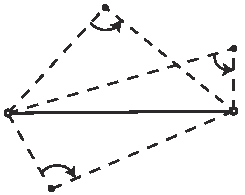
\includegraphics[width=0.22\textwidth]{figures/chap4_chatu_angles.pdf}
  \vspace{-1.2\baselineskip}
\end{wrapfigure}
\tr{式 \eqref{equ:qry-final-expression} 十分简洁，其中每一项都可几何解释为复平面中向量 $(0-\omega_k)$ 与 $(1-\omega_k)$ 的夹角。
此外，\eqref{equ:qry-final-expression} 还可改写为另一种表达，这也是 \cite{Spainhour2024RobustCQ} 的核心动机。}
\tr{根据 Vieta 定理，有：
\begin{equation}
\frac{c(1)}{c(0)} = \frac{a_n \prod_{i=1}^n (1 - \omega_i)}{a_0} = \frac{\prod_{i=1}^n (1 - \omega_i)}{\prod_{i=1}^n (-\omega_i)}.
\end{equation}
因此，式 \eqref{equ:qry-final-expression} 可改写为
\begin{equation}\label{equ:qry-expression_Int}
    w_{\gamma }(\mq)=\frac{1}{2 \pi}\operatorname{Im} \left(\log\left( \frac{c(1)}{c(0)}\right) \right) + K,
\end{equation}
其中 $K \in \mathbb{Z}$ 是由对数多值性引入的整数补偿项。
事实上，\(K\) 正是闭合图形的整数环绕数，而 \(\frac{1}{2\pi}\operatorname{Im}\log(\frac{c(1)}{c(0)})\) 是“闭合补线”对应的环绕数（见图 5）。
}

\begin{figure}[t]
  \centering
  \begin{overpic}[width=0.99\linewidth]{figures/chap4_new_expression.pdf}
    {
 \put(28.5,13){ =}
 \put(59.5,13){ +}
    }
  \end{overpic}
  \vspace{-2mm}
  \caption{
  \tr{GWN 数值可表示为：闭合补线的环绕数（中）加上未知整数项（右）。}
  }
  \vspace{-2mm}
  \label{fig:qry-new_expression}
\end{figure}

\eqref{equ:qry-gene_expression} 的计算不可行当且仅当：
(1) 存在 $j\neq k$ 使得 \(\omega_k=\omega_j\) 或 \(\omega_k=\omega_j^*\)；
(2) \(\text{Im}(\omega_k)=0\)（对应边界情形）。
我们将分别讨论这两种特殊情况，\tr{并说明式 \eqref{equ:qry-final-expression} 仍然成立}。

\paragraph{特殊根}
在实际区域内极少数点处会出现重根，即 \(\omega_k=\omega_j\) 或 \(\omega_k=\omega_j^*\)。
例如当 $n=2$ 时，每条 \Bezier 曲线都是某抛物线的一部分。
条件 \(\omega_1=\omega_2\) 表示查询点位于该抛物线焦点。
更高次时，若多项式曲线满足某些代数条件，也会在类似焦点的特定位置出现重根。
虽然我们在实践中尚未遇到该情况，但仍给出其计算形式。
\(\omega_k\) 与 \(\omega_k^*\) 均为 $m$ 阶极点，且有：
\begin{equation}\label{equ:qry-repeated_expression}
\begin{aligned}
    &\res(G(t),\omega_k)+\res(G(t),\omega_k^*)\\
    &=2 \re \left(\frac{1}{(m-1)!}\lim_{t\to \omega_k}\frac{d^{m-1}}{dt^{m-1}}\{(t-\omega_k)^m G(t)\} \right)\\
    &\tr{=m \im\left(\log\left(1-\frac{1}{w_k}\right)\right)},
    \end{aligned}
\end{equation}
\tr{其中最后一个等式由代入 \eqref{equ:qry-f} 并进行初等化简得到。\eqref{equ:qry-repeated_expression} 说明在特殊根情形下，\eqref{equ:qry-final-expression} 仍然有效。}

\subsection{边界上的 GWN}\label{sec:qry-forboundary}
\paragraph{实根}
若查询点 $\mq$ 位于 \Bezier 曲线上，这里不区分其位于曲线实际段还是位于延拓的多项式曲线上。此时 \(w_k\) 为实数，并且是多项式 \(h(t)\) 的重根。
我们发现，根的具体重数\tr{不影响表达式~\eqref{equ:qry-closed_form_expr} 与计算式~\eqref{equ:qry-final-expression} 的有效性}。
\begin{theorem}\label{pro:qry-boundary}
若 \(w_k\) 为实数，则有：
\[\res(G(t),\omega_k)=0.\]
\end{theorem}
\begin{proof}
一般地，设 \(\omega_k\) 是 \(h(t)\) 的 \((2m)\) 阶根，且 $h(t)=(t-w_k)^{2m}h_e(t)$。由于 \(\omega_k\) 为实数，有
\begin{equation}\label{equ:qry-factorization}
    x(t)=(t-\omega_k)^m x_e(t),y(t)=(t-\omega_k)^m y_e(t),
\end{equation}
\tr{其中 \(h_e(t),x_e(t),y_e(t)\) 为因式分解后的多项式。}由式 \eqref{equ:qry-factorization} 可得
 \begin{equation}
      f(t) = (t-\omega_k)^{2m} (x_e(t)y'_e(t)-y_e(t) x'_e(t)).
 \end{equation}
 由留数公式，得到：
\begin{equation}
\begin{aligned}
    &\res(G(t),\omega_k)=\lim_{t\to \omega_k}\frac{d^{2m-1}}{dt^{2m-1}}\{(t-\omega_k)^{2m} G(t)\} \\
    &=\lim_{t\to \omega_k}\frac{d^{2m-1}}{dt^{2m-1}}\{\frac{f(t)\log(1-\frac{1}{t})}{h_e(t)}\} =0.
 \end{aligned}
\end{equation}
\end{proof}


\paragraph{另一种理解}
定理~\ref{pro:qry-boundary} 的有效性也可从更直观角度理解。当 \(w_k\) 为实数时，可化简为：
\begin{equation}\label{equ:qry-alte_understanding}
    \frac{f(t)}{h(t)}=\frac{x_e(t)y'_e(t)-y_e(t)x'_e(t)}{x_e(t)^2+y_e(t)^2}.
\end{equation}
式~\eqref{equ:qry-alte_understanding} 可视为一条低次 \Bezier 曲线 $\{x_e(t),y_e(t)\}$ 的 GWN，相当于根 \(w_k\) 不存在。

这一观察与我们对边界点 GWN 的理解一致。在线段情形中，GWN 从一侧逼近为 \(+\tfrac{1}{2}\)，从另一侧逼近为 \(-\tfrac{1}{2}\)，因此线段上的点环绕数应为 0~\cite{Jacobson2013RobustIS}。
受此启发，若点位于曲线上，计算环绕数时将曲线划分为三段（若点是端点则为两段）：点附近无穷小邻域对应的曲线段，以及其余部分。无穷小邻域内曲线局部近似线段，对环绕数贡献为 0；因此仅需计算其余两段 \Bezier 曲线的环绕数，因为目标点不位于这两段上，可用常规环绕数计算处理，如图~\ref{fig:qry-boundary} 所示。

\paragraph{边界点判定}
为实现严格几何一致性，文献~\cite{Spainhour2024RobustCQ} 已给出有理曲线端点处 GWN 的计算方法。在此基础上，我们进一步给出曲线上任意点 GWN 的通用计算方法。
仍有一个关键问题：判定给定点是否在有理曲线上。该问题以及点到曲线最短距离问题，通常都可转化为多项式方程求根。
这类问题可用数值方法~\cite{Mortenson1985GeometricM} 或基于控制多边形的裁剪算法~\cite{Ma2003PointIA} 解决；而借助距离函数 \(h(t)\)，我们无需额外操作。
\begin{theorem}\label{pro:qry-near_boundary}
我们有如下结论：
\begin{enumerate}
    \item 当且仅当 $\im(\omega_k)=0$ 时，$\mq$ 位于边界上。
    \item 若 \(\omega_k = a + b i\) 且 \(|b| \ll 1\)，则说明点 \(\mq\) 靠近 \(\gamma(a)\)。此外，当 \(b>0\) 时 \(\mq\) 位于 \(\gamma(a)\) 左侧；当 \(b<0\) 时位于其右侧。
\end{enumerate}
\end{theorem}
\begin{proof}
结论 (1) 易验证，故仅证明 (2)。回顾 \eqref{equ:qry-root-decompose} 中 \(\omega_k\) 的计算，将 \(t=a+bi\) 代入方程 \(x(t)+y(t)i=0\)，得到：
\begin{equation}
    x(a)+y(a)i+b( x'(a)i-y'(a))+b^2(X)=0,
\end{equation}
其中 \(X\) 包含若干未展开项。
由于 \(b \ll 1\)，可忽略项 \(b^2(X)\)，从而得到：
\begin{equation}\label{equ:qry-app_imag}
x(a) \approx b y'(a), \quad y(a) \approx -b x'(a).
\end{equation}
注意 \((x'(a),y'(a))\) 是曲线在 \(\gamma(a)\) 处的有限长度切向量，\((x(a),y(a))\) 是从点 \(q\) 指向 \(\gamma(a)\) 的位移向量，因此 (2) 得证。
\end{proof}

\begin{figure}[t]
  \centering
  \begin{overpic}[width=1.0\linewidth]{figures/chap4_boundary.pdf}
    {
 \put(8,-3){\small \textbf{(a)}}
 \put(39,-3){\small \textbf{(b)}}
 \put(76,-3){\small \textbf{(c)}}
    }
  \end{overpic}
  %\vspace{-2mm}
  \caption{
  (a) 边界点处 GWN 计算（上）仅考虑该点两侧两段曲线（下）。(b) 在整个区域采样点的 GWN。 (c) 在曲线上采样点的 GWN。
  }
  \label{fig:qry-boundary}
\end{figure}

\subsection{GWN 的导数}\label{sec:qry-derivative}
我们还可以计算 GWN 的导数。记：
\begin{equation}
    \frac{\partial w_{\Gamma}(\mq)}{\partial \mq}=\frac{1}{2 \pi} \left(\int_0^1\frac{f_1(t)}{h(t)^2}\,dt,\int_0^1\frac{f_2(t)}{h(t)^2}\,dt\right)
\end{equation}
其中 $f_1 =-2 x' x y +y' (x ^2-y ^2)$，$f_2 =2y' x y +x' (x ^2-y ^2)$。与定理~\ref{pro:qry-general} 类似，可推得：
\begin{equation}
    \int_0^1\frac{f_l(t)}{h(t)^2}\,dt=\sum_{k=1}^n2\re\left(\res(\frac{f_l(t)}{h(t)^2}\log(1-\frac{1}{t}),\omega_k)\right),\  l=1,2.
\end{equation}

在 \cite{Scrivener2024WindingNF} 中，环绕数总变分被用于度量艺术家草图的方向并构建分割框架，如图~\ref{fig:qry-reorientation} 所示。其方法将曲线离散为分段线段后再计算总变分与 GWN 导数。相比之下，我们的方法可更直接地计算这些导数，同时提升效率与精度。

导数计算流程与 GWN 计算类似（见算法~\ref{alg:qry-encoding}），核心步骤是在不同根处评估分子多项式。


\begin{algorithm}[t]
  \caption{WindingNumber\Bezier：计算任意 \Bezier 曲线的广义环绕数}\label{alg:qry-encoding}
  \SetKwInput{KwInput}{输入}
  \SetKwInput{KwOutput}{输出}
  \SetKwFunction{FMain}{Main}
  \SetKwFunction{FD}{D}
  
  \KwInput{\(\Gamma\)：\Bezier 曲线 $\Gamma$\\
          \quad\quad\quad  \(q\)：查询点}
  \KwOutput{$w_\Gamma$：点 $q$ 处的环绕数值}
  % Algorithm
  \tr{
  计算 \(x(t)\) 与 \(y(t)\) 的系数 $\{x_k\}_{k=0}^{n}$ 与 $\{y_k\}_{k=0}^{n}$\;
  $\{\omega_k\}_{k=1}^n \gets$  CalculateRoots$( \{x_k+i y_k\}_{k=0}^n)$\;
 \For{$k \gets 1$ \KwTo $n$}{
    $R[k] \gets \im\left( \log(1-\frac{1}{\omega_k}) \right) \ \text{\bf if} \ |\im(\omega_k)| \geq \epsilon_1 \ \text{\bf else} \ 0$\;
 } 
 }
 \tr{
 \(w_L\gets\frac{1}{2 \pi}\im \left(\log(\frac{x(1)+y(1) i}{x(0)+y(0)i})\right)\);
  \(w_\Gamma\gets\frac{1}{2 \pi}\sum_{k=1}^{n} R[k]\);
 }

 \tr{
 $w_\Gamma\gets\text{ROUND}\left[w_\Gamma-w_L\right]+w_L.$
 }
\end{algorithm}

\begin{algorithm}[t]
  \caption{CalculateRoots：计算复系数多项式的根}\label{alg:qry-encoding2}
  \SetKwInput{KwInput}{输入}
  \SetKwInput{KwOutput}{输出}
  \SetKwFunction{FMain}{Main}
  \SetKwFunction{FD}{D}
  
  \KwInput{\(\{x_k+i y_k\}_{k=0}^n\)：多项式 $c$ 的系数
        }
  \KwOutput{\(\{\omega_k\}_{k=1}^n\)：多项式的根}
  % Algorithm
  \tr{
 $\{\omega_k\} \gets \text{analytical\_solution} \ \text{\bf if} \ n \leq 4 \ \text{\bf else} \ \text{numerical\_solution}$\;
 \For{$k \gets 1$ \KwTo $n$}{
    \While{$\im(\omega_k)<\epsilon_2$ and $|\Delta\omega_k|<\epsilon_3$}{
    $\Delta\omega_k\gets c(\omega_k)/c'(\omega_k)$\;
    \(\omega_k\gets \omega_k-\Delta\omega_k\)\;
    }
 } 
 }
\end{algorithm}

\begin{figure}[t]
  \centering
  \begin{overpic}[width=0.99\linewidth]{figures/chap4_reoritation.pdf}
    {
    }
  \end{overpic}
  \vspace{-4mm}
  \caption{
  左：艺术家原始草图的 GWN 结果，图中两笔均按逆时针绘制，体现了笔画方向被忽略的情况。
  右：重定向后草图的 GWN 结果。
  }
  \label{fig:qry-reorientation}
\end{figure}


\section{实验与评估（Query）}\label{sec:qry-results}
我们的方法采用 C++ 实现。所有实验在一台配备 4.00 GHz Intel Core i7-4790K 处理器和 16 GB 内存的台式机上完成。算法中唯一由用户控制的参数是容差 \(\epsilon_1\)，用于定义查询点 \(\mq\) 与边界曲线距离多近时可被视为位于曲线上。所有实验统一设定 $\epsilon_1=10^{-16}$（图~\ref{fig:qry-gallery}）。

\begin{figure}[t]
  \centering
  \begin{overpic}[width=1.0\linewidth]{figures/chap4_diff_order.pdf}
    {
    \put(20,-3){\small 总时间: 0.16s vs. 1.10s}
    \put(62,-3){\small 总时间: 1.25s vs. 1.85s}
    }
  \end{overpic}
  \caption{
 左：两条二次有理曲线（含四分之一椭圆与负权重的四分之三椭圆）的 GWN。
 右：五次有理曲线的 GWN。
 图下文字给出了本文方法与 \cite{Spainhour2024RobustCQ} 的总计算时间。
  }
  \vspace{-3mm}
  \label{fig:qry-diff-order}
\end{figure}

\begin{figure}[t]
  \centering
  \begin{overpic}[width=0.99\linewidth]{figures/chap4_round.pdf}
    {
    }
  \end{overpic}
  \vspace{-4mm}
  \caption{
  不同情形下的取整 GWN。
  }
  \vspace{-3mm}
  \label{fig:qry-round}
\end{figure}


\begin{figure*}[t]
  \centering 
  \begin{overpic}[width=0.96\linewidth]{figures/chap4_gallery.pdf}
    {
    }
  \end{overpic}
  \vspace{-4mm}
  \caption{
  各类复杂模型的 GWN 可视化结果，颜色映射见右下角色条。
  }
  \label{fig:qry-gallery}
\end{figure*}

\tr{
\paragraph{数值稳定性}
我们对 \eqref{equ:qry-final-expression} 采用如下计算形式：
\begin{equation}\label{equ:qry-actual_expression}
    \im(\log(1-\frac{1}{\omega_k}))=\text{atan2}(\im(\omega_k),\|\omega_k\|^2-\re(\omega_k)).
\end{equation}
仅当 \(\|\omega_k\|^2-\re(\omega_k)=0\) 时，\(\arctan(\cdot)\) 不适定；这等价于 \(\omega_k=0\) 或 \(\omega_k=1\)（即 \(\mq\) 位于 \(\gamma\) 的端点）。命题~\ref{pro:qry-boundary} 说明此时该值可置为 0。
}

\tr{
将式~\eqref{equ:qry-final-expression} 用于计算时，唯一误差来源是求根过程。为消除该误差，一种简单有效的做法是先估计未知整数项 \(K\)，再用 \eqref{equ:qry-expression_Int} 进行计算。具体如算法~\ref{alg:qry-encoding} 的编码流程所示：将 \((w_\Gamma-w_L)\) 四舍五入到最近整数后再加回 \(w_L\)，即可得到与 \(w_L\) 同精度级别的 \(w_\Gamma\)。
}

\tr{
仅存在一种例外情况：当 \(\omega_k\) 的实部位于 $(0,1)$ 且求根误差导致 \(\im(\omega_k)\) 符号翻转时，命题~\ref{pro:qry-near_boundary} 表明查询点极接近曲线，此时解析计算可能给出错误的内外判定。
为增强数值鲁棒性，当遇到虚部低于阈值 \(\epsilon_2=10^{-12}\) 的根时，可执行牛顿细化，直到 \(\im(\omega_k)\) 的变化小于 \(\epsilon_3=10^{-18}\)（见算法~\ref{alg:qry-encoding2}）。
}

\paragraph{不同次数}
三次 \Bezier 曲线是 PostScript 与 SVG 格式所要求的最高次数，通常已足够表达设计细节。
不过，在配合数值求根算法~\cite{Skowron2012} 时，我们的方法同样适用于更高次数曲线。
如图~\ref{fig:qry-diff-order} 所示，我们对五次有理曲线计算 GWN，在保持精确评估的同时，速度仍快于 \cite{Spainhour2024RobustCQ}。
此外，即使是具有负权重、不满足凸包性质的有理曲线（\cite{Spainhour2024RobustCQ} 无法处理），我们的闭式表达仍然有效。
整体速度主要取决于不同次数下求根过程的效率。

\paragraph{取整环绕数}
GWN 的小数部分可被视作包含查询置信度的一种度量。
如图~\ref{fig:qry-round} 所示，将每个 GWN 值四舍五入到最近整数后，可形成一个环绕数字段。基于该字段的取整过程会产生三种边界近似，并在局部消除相交或断开曲线对包含判定的影响。

\paragraph{大规模评估}
\tr{我们在 OpenClipArt 数据集~\cite{hu2019TriWild}（含 17,944 个真实 SVG）上进行了大规模定量评估。虽然较少见，但数据集中有些曲线会出现“实际多项式次数”与“控制点数量”不匹配的情况，可能源于低次 \Bezier 曲线的升阶。在算法中，这体现为多项式 \(c(t)\) 的首项系数接近 0。实践中，当首项系数绝对值小于阈值 \(\epsilon_4=10^{-12}\) 时，我们切换到低一阶求根公式，并显式将一个根设为 0。}

\tr{为更本质地评测求根子程序的精度与稳定性，我们同时使用式~\eqref{equ:qry-final-expression} 和式~\eqref{equ:qry-expression_Int} 进行计算。
由于本文方法与 \cite{Spainhour2024RobustCQ} 都使用了多次 \text{atan2} 运算，而本文额外使用了求根公式，因此我们将“式~\eqref{equ:qry-final-expression} 与 \cite{Spainhour2024RobustCQ} 结果差异”视为求根过程引入误差的度量。}

\begin{figure}[t]
  \centering
  \begin{overpic}[width=0.99\linewidth]{figures/chap4_dataset.pdf}
    {
    }
  \end{overpic}
  \vspace{-3mm}
  \caption{
  \tr{我们进行了大规模矢量图评测。
  左图给出本文方法（使用式~\eqref{equ:qry-expression_Int}）与 \cite{Spainhour2024RobustCQ} 的时间比。
  右图给出本文结果（蓝：式~\eqref{equ:qry-expression_Int}；紫：式~\eqref{equ:qry-final-expression}）相对于 \cite{Spainhour2024RobustCQ} 的绝对差值。
  在所有图形上，我们都取得更短计算时间，但随着曲线数量增加，领先幅度会缩小。
  求根过程会在少量接近“升阶退化”曲线上引入误差，本实验中最大误差为 \(2.1\times 10^{-3}\)。}
  }
  \label{fig:qry-dataset}
\end{figure}


\begin{figure*}[t]
  \centering
  \begin{overpic}[width=0.98\linewidth]{figures/chap4_compare_result_simp.pdf}
    {
    \put(8,-1){\small 原始形状}
    \put(32,-1){\small GWN 数值}
    \put(52,-1){\small \cite{Spainhour2024RobustCQ}}
 \put(81,-1){\small 本文方法}
  \put(99,1){\small \rotatebox{90}{单点运行时间($\mu s$)}}
  \put(59,20.7){\small 总时间: 3.32s}
  \put(82.5,20.7){\small 总时间: 1.66s}
  \put(59,1){\small 总时间: 1.22s}
  \put(82.5,1){\small 总时间: 0.77s}
    }
  \end{overpic}
  \vspace{-1mm}
  \caption{
  在两个模型上与~\cite{Spainhour2024RobustCQ} 的比较，GWN 值使用图~\ref{fig:qry-gallery} 的色条可视化。
  对于曲线包围盒外部区域，两种方法采用相同计算策略。
  }
  \vspace{-1mm}
  \label{fig:qry-cmp}
\end{figure*}

\tr{
在每个图形的包围盒内部，我们随机采样 10,000 个点，记录平均计算时间以及本文结果与 \cite{Spainhour2024RobustCQ} 结果的最大差值，如图~\ref{fig:qry-dataset} 所示。式 \eqref{equ:qry-final-expression} 出现较大数值误差的少量案例，通常源于首项系数仅略大于 \(\epsilon_4\) 的曲线。
}

\paragraph{与 \cite{Spainhour2024RobustCQ} 的比较}
我们在每个示例的单位正方形内均匀采样 100 万个点，并与 \cite{Spainhour2024RobustCQ} 比较总计算时间。
当采样点位于曲线包围盒外时，我们采用与对方相同的计算方式。
在查询点位于曲线包围盒内部时，对于二次与三次曲线，本文方法可达到约 $7\times$ 的速度优势；而在更高次曲线上该优势会减弱。
对于更复杂模型（见图~\ref{fig:qry-dataset} 与图~\ref{fig:qry-cmp}），随着模型中曲线尺寸变小，我们的性能领先也会下降。这是因为对多数点而言，两种方法的评估过程差异不大。
\tr{例如在图~\ref{fig:qry-cmp} 的两个案例中，仅有 2.4\% 和 1.9\% 的计算发生在曲线包围盒内，而绝大多数评估发生在包围盒外。}
